%%% CSE 4316 Individual Sprint Report - WORKED EXAMPLE (Autonomous Ground Robot)
\documentclass{article}
\usepackage{siunitx}\usepackage{graphicx}\usepackage{amsmath}
\setlength\parindent{0pt}
\usepackage[letterpaper, portrait, margin=1in]{geometry}

\title{Sprint 3 Report \\ CSE 4316}
\author{Ada Lovelace}
\date{November 3rd, 2026}

\begin{document}
\maketitle
\begin{center}
\begin{tabular}{l r}
Sprint start date: & October 20th, 2026 \\
Sprint end date: & November 3rd, 2026 \\
Project title: & TerraScout Autonomous Ground Rover \\
Team name: & Team Trailblazer \\
Partners: 	& Alan Turing \\
			& Grace Hopper \\
			& John Von Neumann \\
        	& Charles Babbage \\
Instructor: & Christopher D. McMurrough
\end{tabular}
\end{center}

\section{Sprint Goal}
Stand up the perception pipeline: synchronized RGB/thermal capture tagged with pose,
and a first fault-detection baseline evaluated against the sponsor validation set.

\section{Sprint Backlog}
Breakdown of planned tasks assigned to the team (work units in hours). \\
\begin{tabular}{| p{4in} | >{\centering\arraybackslash} p{1in} | >{\centering\arraybackslash} p{1in} |}
\hline
\textbf{Task description} & \textbf{Estimated work} & \textbf{Actual work} \\ \hline
Integrate thermal camera driver (ROS 2 node) & 6.0 & 8.0 \\ \hline
Hardware trigger for RGB/thermal sync & 4.0 & 5.0 \\ \hline
Pose stamping of captured frames & 3.0 & 2.5 \\ \hline
Label sponsor validation set & 5.0 & 4.0 \\ \hline
Train MobileNet baseline detector & 6.0 & 7.0 \\ \hline
Evaluate detector (precision/recall) & 3.0 & 3.0 \\ \hline
Ground-station telemetry stub & 4.0 & 3.5 \\ \hline
\textbf{TOTAL} & \textbf{31.0}  & \textbf{33.0} \\ \hline
\end{tabular}

\pagebreak

\section{Individual Time Expenditures}
Summary of tasks performed by the individual (hours). \\
\begin{tabular}{| p{4in} | >{\centering\arraybackslash} p{1in} | >{\centering\arraybackslash} p{1in} |}
\hline
\textbf{Task Description} & \textbf{Actual work} & \textbf{Percent complete} \\ \hline
Label sponsor validation set & 4.0 & 100\% \\ \hline
Train MobileNet baseline detector & 7.0 & 100\% \\ \hline
Evaluate detector (precision/recall) & 3.0 & 100\% \\ \hline
Investigate thermal false positives & 2.0 & 60\% \\ \hline
\textbf{TOTAL} & \textbf{16.0}  & \textbf{-} \\ \hline
\end{tabular}

\section{Team Burndown Chart}
Ideal (baseline) and actual daily team effort are shown below.
\begin{figure}[h]\begin{center}
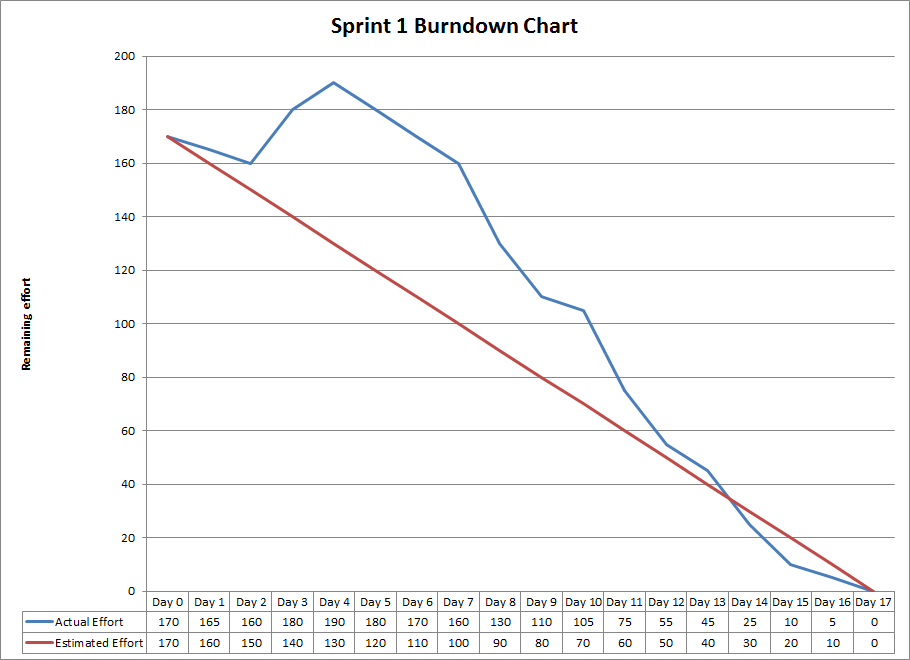
\includegraphics[width=1.0\textwidth]{images/burndown}
\end{center}\end{figure}

\pagebreak

\section{Individual Retrospective}
The following describe actions to start, stop, or continue next sprint. \\

Actions to \textbf{start} doing (top 3)
\begin{itemize}
\item Version-control trained model artifacts with dataset hashes for reproducibility.
\item Write the evaluation script first, before training, to fix the metric.
\item Book the outdoor test slot at the start of the sprint, not the end.
\end{itemize}

Actions to \textbf{stop} doing (top 3)
\begin{itemize}
\item Hand-tuning thresholds in a notebook instead of in the node config.
\item Committing large raw thermal captures to Git (use the shared drive).
\item Estimating CV tasks without a data-labeling sub-estimate.
\end{itemize}

Actions to \textbf{continue} doing (top 3)
\begin{itemize}
\item Pairing with John on the pose-stamping interface.
\item Daily short syncs on integration blockers.
\item Keeping the detector behind a stable, replaceable model interface (QA-01).
\end{itemize}

\section{Peer Review}
Candid individual assessment; not shared with other members. Each item graded 1--5. \\

Evaluation items:
\begin{itemize}
\item \textbf{Participation} - present and contributing to goals and tasks?
\item \textbf{Communication} - timely updates; effective use of team tools?
\item \textbf{Work quality} - claimed backlog tasks; met objectives; added value?
\item \textbf{Professionalism} - professional, collaborative, taking it seriously?
\item \textbf{Overall} - overall value to the project this period.
\end{itemize}

\begin{tabular}{| p{1.5in} | >{\centering\arraybackslash} p{1.in} | >{\centering\arraybackslash} p{1.1in} | >{\centering\arraybackslash} p{1.1in}| >{\centering\arraybackslash} p{0.5in}| >{\centering\arraybackslash} p{.5in} |}
\hline
\textbf{Team member name} & \textbf{Participation} & \textbf{Communication} & \textbf{Work quality} & \textbf{Professionalism} & \textbf{Overall} \\ \hline
Ada Lovelace & 5 & 5 & 5 & 5 & 5\\ \hline
Alan Turing & 5 & 4 & 5 & 5 & 5\\ \hline
Grace Hopper & 5 & 5 & 4 & 5 & 5\\ \hline
John Von Neumann & 4 & 4 & 5 & 4 & 4\\ \hline
Charles Babbage & 4 & 3 & 4 & 4 & 4\\ \hline
\end{tabular}

\end{document}
